\section{Indutores em C.C. e C.A.}

\frame{
	\frametitle{O Indutor}
	\begin{block}{Introdução}
		Um indutor é um dispositivo elétrico passivo que armazena energia na forma de campo magnético, normalmente combinando o efeito de vários loops da corrente elétrica.
	\end{block}

	\bigskip
	
	\centerline{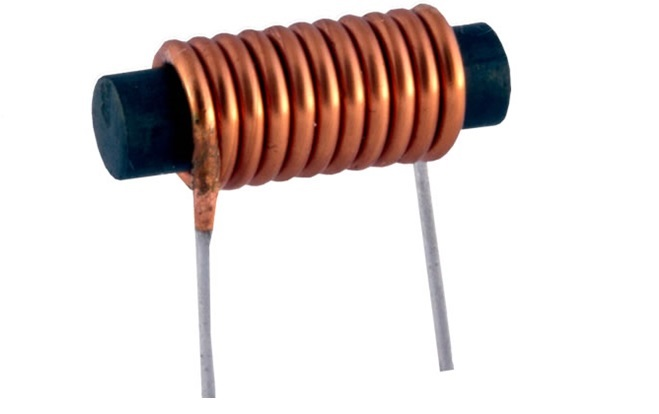
\includegraphics[width=0.5\linewidth]{Figuras/Ch13/Indutores.jpg}}
}

\frame{
	\frametitle{Indutância}
	\begin{block}{Aspectos construtivos}
		\begin{itemize}
			\item Indutância ($L$) determina a força do campo magnético em torno da bobina por causa de uma corrente aplicada.
			\item O nível de indutância tem sensibilidades de construções similares, no sentido de que ele é dependente da área dentro da bobina, do comprimento da unidade e da permeabilidade do material do núcleo.
			\item Ele também é sensível ao número de espiras na bobina.
		\end{itemize}
	\end{block}
}

\frame{
	\frametitle{Indutância}
	\begin{block}{Relação matemática}
		$$L =  \dfrac{N^2 \mu A}{l} \qquad [\si{\henry}]$$
	\end{block}
}

\frame{
	\frametitle{Transitório: fase de carga}
	\setmyunit{2cm}
	\centering
	\begin{circuitikz}[european voltages]
		\draw (0,0) to[R,l=$ R $,v=$ v_R $,i=$ i $,o-] ++(1.5,0)
		to[L,l=$ L $,v=$ v_L $,i=$ i_L $] ++(0,-1)
		to[short,-o] ++(-1.5,0);
		\draw[decorate,decoration={brace,amplitude=10pt,mirror},xshift=-5pt] (0,0) -- node[left=8pt] {$ U $} (0,-1);
	\end{circuitikz}
	
%	\centerline{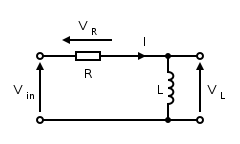
\includegraphics[width=0.6\linewidth]{Figuras/Ch13/indutorcc.png}}
	\begin{block}{Indutor em regime C.C.}
		\begin{itemize}
			\item O que é verdadeiro para a tensão de um capacitor também é verdadeiro para a corrente de um indutor, e o que é verdadeiro para a corrente de uma capacitor pode ser igualado de muitas maneiras pela tensão de um indutor.
			\item As formas de onda de armazenamento têm o mesmo formato.
		\end{itemize}
	\end{block}
}

\frame{
	\frametitle{Transitório: fase de carga}
	\setmyunit{2cm}
	\centering
	\begin{circuitikz}[european voltages]
		\draw (0,0) to[R,l=$ R $,v=$ v_R $,i=$ i $,o-] ++(1.5,0)
		to[L,l=$ L $,v=$ v_L $,i=$ i_L $] ++(0,-1)
		to[short,-o] ++(-1.5,0);
		\draw[decorate,decoration={brace,amplitude=10pt,mirror},xshift=-5pt] (0,0) -- node[left=8pt] {$ U $} (0,-1);
	\end{circuitikz}

%	\centerline{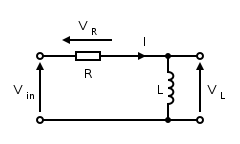
\includegraphics[width=0.6\linewidth]{Figuras/Ch13/indutorcc.png}}
	\begin{block}{$t=0$}
		\begin{itemize}
			\item No instante em que a chave é fechada, a bobina evita uma variação instantânea na corrente, o que resulta em $i_L = \SI{0}{\ampere}$.
			\item A ausência de corrente através da bobina e do circuito resulta em \SI{0}{\volt} através do resistor, portanto a tensão no indutor é máxima.
		\end{itemize}
	\end{block}
}

\frame{
	\frametitle{Transitório: fase de carga}
	\setmyunit{2cm}
	\centering
	\begin{circuitikz}[european voltages]
		\draw (0,0) to[R,l=$ R $,v=$ v_R $,i=$ i_R $,o-] ++(1.5,0)
		to[L,l=$ L $,v=$ v_L $,i=$ i_L $] ++(0,-1)
		to[short,-o] ++(-1.5,0);
		\draw[decorate,decoration={brace,amplitude=10pt,mirror},xshift=-5pt] (0,0) -- node[left=8pt] {$ U $} (0,-1);
	\end{circuitikz}

%	\centerline{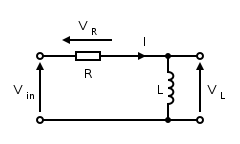
\includegraphics[width=0.6\linewidth]{Figuras/Ch13/indutorcc.png}}
	\begin{block}{$t=0^+$}
		\begin{itemize}
			\item Inicialmente, a corrente aumenta muito rapidamente.
			\item A tensão através do resistor aumenta na mesma medida, porque $v_R = i_R \cdot R = i_L \cdot R$.
		\end{itemize}
	\end{block}
}

\frame{
	\frametitle{Transitório: fase de carga}
	\setmyunit{2cm}
	\centering
	\begin{circuitikz}[european voltages]
		\draw (0,0) to[R,l=$ R $,v=$ V_R $,i=$ i $,o-] ++(1.5,0)
		to[L,l=$ L $,v=$ V_L $,i=$ i_L $] ++(0,-1)
		to[short,-o] ++(-1.5,0);
		\draw[decorate,decoration={brace,amplitude=10pt,mirror},xshift=-5pt] (0,0) -- node[left=8pt] {$ U $} (0,-1);
	\end{circuitikz}

%	\centerline{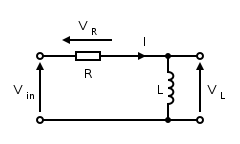
\includegraphics[width=0.6\linewidth]{Figuras/Ch13/indutorcc.png}}
	\begin{block}{$t=\infty$}
		\begin{itemize}
			\item Por fim, quando a corrente alcança seu valor de estado estacionário, a variação da corrente através da bobina cessa.
			\item Com o fim da variação da corrente, a tensão cai para \SI{0}{\volt}.
		\end{itemize}
	\end{block}
}

\frame{
	\frametitle{Constante de tempo}
	\centerline{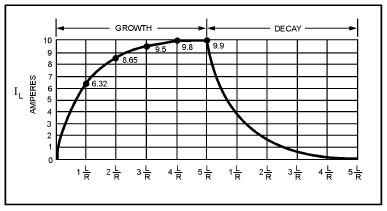
\includegraphics[width=0.7\linewidth]{Figuras/Ch13/ctetempo2.png}}
	\begin{block}{Constante de tempo}
		O fator $\tau$, chamado de constante de tempo do circuito, tem a unidade de tempo e pode ser calculada como:
		
		$$\tau = \dfrac{L}{R}$$
	\end{block}
}

\frame{
	\frametitle{Transitório: fase de carga}
	\centerline{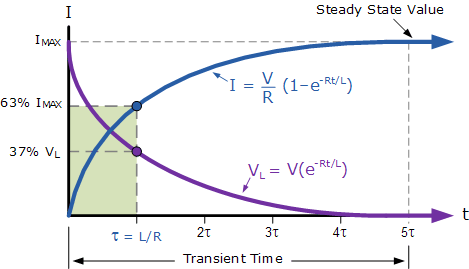
\includegraphics[width=0.6\linewidth]{Figuras/Ch13/tensaocorrentecarga2.png}}
	\begin{block}{Curva de carga - corrente}
		\[ i_L(t) = i\Big( 1-\text{e}^{-t/\tau}\Big) \]
		\begin{itemize}
			\item A corrente de um circuito C.C. indutivo é essencialmente máximo após cinco constantes de tempo da fase de carga terem passado.
		\end{itemize}
	\end{block}
}

\frame{
	\frametitle{Transitório: fase de carga}
	\centerline{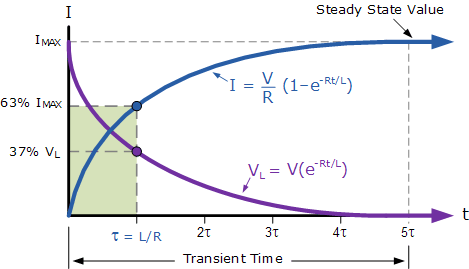
\includegraphics[width=0.6\linewidth]{Figuras/Ch13/tensaocorrentecarga2.png}}
	\begin{block}{Curva de carga - tensão}
		\[ v_L = \epsilon - R \cdot i(t) \implies v_L = \epsilon - R \cdot i\Big( 1-\text{e}^{-t/\tau}\Big) \implies v_L(t) = \epsilon \Big(\text{e}^{-t/\tau}\Big) \]
		\begin{itemize}
			\item A tensão através de um indutor em um circuito C.C. é essencialmente igual à zero após cinco constantes de tempo da fase de carga.
		\end{itemize}
	\end{block}
}

\frame{
	\frametitle{Transitório: fase de carga}
	\begin{block}{Conclusões}
		\begin{itemize}
			\item O indutor assume as características de um circuito aberto no instante em que a chave é fechada.
			\item O indutor assume as características de um curto-circuito quando as condições de estado estacionário são estabelecidas.
		\end{itemize}
	\end{block}
}

\frame{
	\frametitle{Indutores em regime C.A.}
	\begin{block}{Reatância indutiva}
		A reatância indutiva é uma oposição à corrente que resulta em uma troca contínua de energia entre a fonte e o campo magnético do indutor. Sua relação é dada por:
		$$X_L = 2\pi fL \qquad[\si{\ohm}]$$
		\begin{itemize}
			\item À medida que a frequência diminui, a reatância indutiva decresce até atingir um valor praticamente nulo.
		\end{itemize}
	\end{block}
}

\frame{
	\frametitle{Indutores em regime C.A.}
	\begin{block}{Tensão e corrente do indutor}
		Lembrando que quando o indutor está energizado ($v_L = \SI{0}{\volt}$), a corrente
		é máxima; e quando desenergizado ($v_L = V_{\text{máx}}$), a corrente é nula.
	\end{block}
}

\frame{
	\frametitle{Indutores em regime C.A.}
	\begin{block}{Tensão e corrente do indutor}
		$$i(t) = I_{\text{máx}}\cdot \sen \left( \omega t - \dfrac{\pi}{2}\right)  \quad \text{onde } I_{\text{máx}} = \dfrac{V_{\text{máx}}}{X_L}$$
	\end{block}
	\centerline{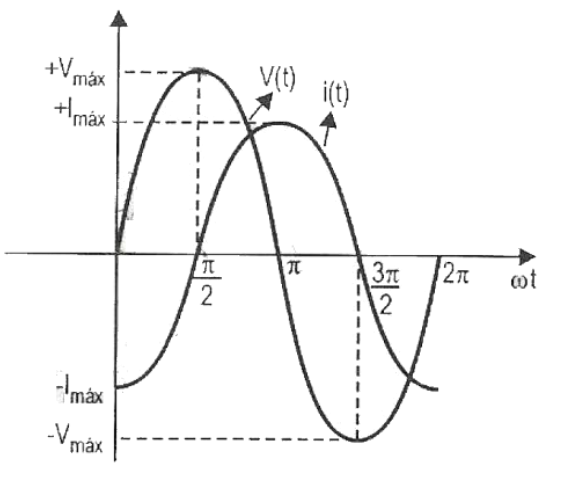
\includegraphics[width=0.45\linewidth]{Figuras/Ch13/tensaocorrente2.PNG}}
	\vspace{-0.5cm}
	\begin{block}{Conclusão}
		Dizemos que a \textbf{corrente está atrasada $\ang{90}$ em relação a tensão.}
	\end{block}
}

\frame{
	\frametitle{Circuitos RL série}
	\setmyunit{2cm}
	\centering
	\begin{circuitikz}
		\draw (1,0) to[sV,l_=$ v $] ++(0,-1.5) -- ++(1.5,0)
		(1,0) to[R,l=$ R $] ++(1.5,0)
		to[L,l=$ X_L $] ++(0,-1.5);
	\end{circuitikz}
%	\centerline{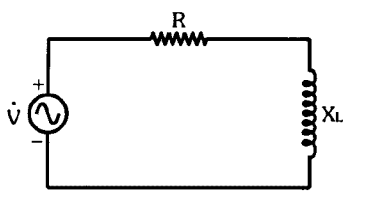
\includegraphics[width=0.6\linewidth]{Figuras/Ch13/rlserie.PNG}}
	\begin{block}{Impedância}
		Todo circuito em regime AC oferece uma oposição à passagem de corrente elétrica denominada impedância ($Z$) medida em ohms ($\si{\ohm}$). No circuito RL série a impedância é a soma vetorial de $R$ e $X_L$.
	\end{block}
}

\frame{
	\frametitle{Circuitos RL série}
	\setmyunit{2cm}
	\centering
	\begin{circuitikz}[scale=0.7]
		\draw (1,0) to[sV,l_=$ v $] ++(0,-1.5) -- ++(1.5,0)
		(1,0) to[R,l=$ R $] ++(1.5,0)
		to[L,l=$ X_L $] ++(0,-1.5);
	\end{circuitikz}

%	\centerline{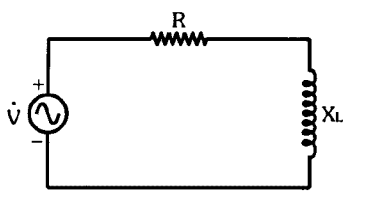
\includegraphics[width=0.4\linewidth]{Figuras/Ch13/rlserie.PNG}}
	\begin{block}{Formulações}
		\begin{gather*}
			Z = \sqrt{R^2 + X_L^2}\\
			\phi = \arctg \left( \dfrac{X_L}{R} \right) \\
			I_{\text{ef}} = \dfrac{V_{\text{ef}}}{Z}\\
			V_{\text{Ref}} = R \cdot I_{\text{ef}}\\
			V_{\text{Lef}} = X_L \cdot I_{\text{ef}}
		\end{gather*}
	\end{block}
}

\section*{Exercícios}

\frame{
	\frametitle{Exercícios}
	\begin{block}{}
		01. Esboce o diagrama vetorial de um circuito RL série considerando uma fonte de tensão alternada de \SI{100}{\voltef} com frequência \SI{60}{\hertz}, $L = \SI{0.5}{\henry}$ e $R = \SI{100}{\ohm}$.

		\vspace{1cm}

		02. A reatância de um indutor é igual à resistência de um resistor de $ \SI{10}{\kilo\ohm}$ na frequência de \SI{5}{\kilo\hertz}. Qual é a indutância do indutor?

		\vspace{1cm}

		03. Considere um circuito RL série. Seja $\epsilon = \SI{20}{\volt}$, $R = \SI{20}{\kilo\ohm}$ e $L = \SI{300}{\milli\henry}$. (a) Determine a constante de tempo, (b) escreva a expressão matemática para a corrente $i_L$ após a chave ser fechada.

	\end{block}
}

\section*{Referências}

\frame{
	\frametitle{Referências e Exercícios Complementares}
	\begin{itemize}
		\item ALEXANDRE, Charles K.; SADIKU, Matthew N. O. Fundamentos de Circuitos Elétricos. 5. ed. Porto Alegre: AMGH, 2013.
	\end{itemize}
	%\centering{\alert{Página 36 - \textbf{1.6.1 até 1.6.5, 1.6.17 até 1.6.19}}} \\
	\centering{\alert{Lista de exercícios 13}}
}